%
% !BIB TS-program = biber
% !BIB program = biber
% !TeX spellcheck = en_US
% !TeX program = lualatex
%
% v 3.00 Feb 2026   Volker RW Schaa
%   
\documentclass[%	              % the JACoW page size is fixed and a4paper/letterpaper is ignored
               %boxit,        % check whether paper is inside correct margins
               %titlepage,    % separate title page
               %refpage       % separate references
               %biblatex,     % biblatex is used
               %nospread,     % flushend option: do not fill with whitespace to balance columns
               hyphens,       % allow \url to hyphenate at "-" (hyphens)
               %xetex,        % use XeLaTeX to process the file
               %luatex,       % use LuaLaTeX to process the file
               ]{jacow}

\usepackage[english]{babel}
\usepackage{pdfpages}
\usepackage{fancyvrb}
\DefineShortVerb{\★}
\usepackage[version=4]{mhchem}
\usepackage{stfloats}
\usepackage[most]{tcolorbox}
\lstdefinelanguage{none}{}

\newtcblisting{TCbox}{%
				boxrule=.3pt,
				colback=blue!5!white,%
				colframe=blue!75!black, %
				left=1mm,top=1mm, bottom=1mm, right=1mm,
				boxsep=0mm, 
				before skip balanced=0pt, 
				after skip balanced=6pt}

\newtcolorbox{Tbox}{%
				boxrule=.3pt,
				colback=blue!5!white,%
				colframe=blue!75!black, %
				left=1mm,top=1mm, bottom=1mm, right=1mm,
				boxsep=0mm, 
				before skip balanced=0pt, 
				after skip balanced=6pt}
				
\newtcblisting{Tverb}{
				boxrule=.3pt,
				colback=blue!5!white,%
				colframe=blue!75!black, %
				left=1mm,top=1mm, bottom=1mm, right=1mm,
				boxsep=0mm, 
				before skip balanced=0pt, 
				after skip balanced=6pt,
			    listing only,
			    listing options={
			    	language=none,
			    	style=tcblatex,
			    	basicstyle=\ttfamily,
			    	columns=flexible,
			    },
			    every listing line={\small\ttfamily},
			  }
%
% when BibLaTeX is used:
%      Bib file in JACoW must be named like the main file + .bib
%      the file type (.bib) is mandatory
%
\ifboolexpr{bool{jacowbiblatex}}%
 {%
  \addbibresource{\jobname.bib}
  \addbibresource{more-biblatex-bib-files.bib}	% more Bib files may be loaded 
 }{}
%\listfiles

% abbreviation for \textsuperscript (TSP) 
%              and \textsubscript (TSB)
\newcommand{\TSP}[1]{\textsuperscript{#1}}
\newcommand{\TSB}[1]{\textsubscript{#1}}

%
% the following macro is used to switch between UK and US english 
%
\newif\ifjacowLangGB
\jacowLangGBfalse
\newcommand{\Lang}[2]{\ifboolexpr{bool{jacowLangGB}}{#1}{#2}}

%%
%%   Lengths for the spaces in the title
%%   \setlength\titleblockstartskip{..}  %before title, default 3pt
%%   \setlength\titleblockmiddleskip{..} %between title + author, default 1em
%%   \setlength\titleblockendskip{..}    %afterauthor, default 1em


\begin{document}



\title{\NoCaseChange{JACoW} {\LaTeX} Style Guide (\NoCaseChange{v}.2026-02-19)%
		\thanks{Work supported by <funding note>}
		}

		\author[1]{V.\,R.W. Schaa\thanks{\texttt{v.r.w.schaa@gsi.de}}}
		\author[2]{I. Andrian}
		\author[3]{S. Brown Gibbs}
		\author[4]{Z. Chen}
		\author[5]{J. Chrin}
		\affil[1]{GSI Helmholtzzentrum für Schwerionenforschung, Darmstadt, Germany}
		\affil[2]{Elettra Sincrotrone Trieste, Basovizza, Italy}
		\affil[3]{Oak Ridge National Laboratory, Oak Ridge, TN, USA}
		\affil[4]{Shanghai Advance Research Institute, CAS, Shanghai, China}
		\affil[5]{PSI Center for Accelerator Science and Engineering, Villigen, Switzerland}

\maketitle


\begin{abstract}
	Many accelerator-related conference series have adopted the same standards 
	for electronic publication and have joined the Joint Accelerator Conferences Website (JACoW) collaboration 
	for the publication of their proceedings. This document describes the requirements 
	for the submission of papers to these conferences and their ultimate publication 
	at \texttt{www.JACoW.org}. 
	Please consult individual conference information for page limits, 
	method of electronic submission, etc. The abstract itself is to act 
	as a stand-alone entity and, as such, should not include numbered reference citations,
	references to pictures, nor footnotes.
	Any acronyms should be expanded on their first occurrence, 
	both in the abstract and in the rest of the paper.
\end{abstract}

\section{SUBMISSION OF PAPERS}

Each author must submit the PDF file and all source files (text, figures, 
bibliographic references) to ensure the paper can be reliably reconstructed 
when there are processing difficulties, errors, or mistakes to be corrected.

\section{MANUSCRIPTS}

This paper serves as a {\LaTeX} style guide for JACoW conferences.
It describes the \LaTeX\ class file and specialties specific to \LaTeX.
A shorter template exemplifying usage of the requirements is also provided for authors.
Please consult \texttt{www.JACoW.org} or the individual conference.

\subsection{General Layout}

The implementation of the layout requirements are realized in
the ‘\texttt{jacow}’ class file (\texttt{\textbf{v3.00}} of 
\texttt{\textbf{2026-02-02}}) and demonstrated in a separate template (see \texttt{jacow-latex-template.tex}). 
As all parameters for page size, margin specifications, 
column layout and balancing are set in the class file, 
Fig.~\ref{fig:paper_layout} only illustrates the layout of the text on the page. 
\begin{figure}[!htb]
   \centering
   \includegraphics*[width=.75\columnwidth]{jacow_pagesize.png}
   \caption{Layout of papers using the ‘\texttt{jacow}’ page size (red box) 
            which is the shorter side of \texttt{A4} (width) and of \texttt{letter} (height) paper.}
   \label{fig:paper_layout}
\end{figure}

The page size option (e.\,g. ‘\texttt{a4paper}’ or ‘\texttt{letterpaper}’)
has no influence on the final size of the generated PDF as it 
is internally set to be the ‘\texttt{jacow}’ page size (red box in Fig.~\ref{tab:page-sizes}); it can therefore be omitted.
Table~\ref{tab:page-sizes} is provided for checking the measures in Acrobat. 
It gives the page width and height in points, millimeter, and inch.
\begin{table}[!hbt]
   \centering
   \caption{Page Size Measures of \texttt{jacow} Class}
   \begin{tabular}{lcc}
       \toprule
       \textbf{Unit} & \textbf{Width} & \textbf{Height} \\ 
       \midrule
           pt     & \qty{595.0}{pt}          & \qty{792.0}{pt}        \\
           mm     & \qty{210.0}{mm}          & \qty{279.5}{mm}        \\
           inch   & \qty{8.26}{inch}         & \qty{11.0}{inch}        \\ 
       \bottomrule
   \end{tabular}
   \label{tab:page-sizes}
\end{table}
\begin{figure*}[!ht]
    \centering
    \includegraphics*[width=.975\textwidth]{jacow_groupphoto_tm2025}

    \caption{Example of a full-width figure showing the JACoW Team at their annual
    	     meeting in 2025 at CERN in Geneva, Switzerland.}
    \label{fig:jacow_team}
%    \vspace*{-\baselineskip}
\end{figure*}

If desired, tables and figures may span the whole \qty{170}{mm} page width 
(2~columns with \qty{82.5}{mm} each plus a gutter of \qty{5}{mm}) as shown
in Fig.~\ref{fig:paper_layout}.

Authors are advised to use {\TeX} names for specifying the width of
embedded material: ★\textwidth★ is equivalent to \qty{170}{mm},
★\columnwidth★ to \qty{82.5}{mm}, ★\linewidth★ is normally equivalent to
★\columnwidth★ but can be used, e.\,g., when a table is embedded in a list environment which by itself
is indented and does not have the full width of the column. 


\subsection{Fonts}

In order to produce portable Adobe Acrobat PDF files, authors are asked 
to use only the fonts defined in the class file in standard, 
bold (i.\,e., ★\textbf★) or italic (i.\,e., ★\textit★) form 
and symbols from the standard set of fonts. The font format should be
\texttt{TrueType} or \texttt{OpenType}.

Authors writing papers containing equations and other mathematical expressions
should make sure that the matching math font set is available. The standard 
setup uses the »\texttt{TeX-Gyre}« fonts which requires the matching math font 
package »\texttt{teX-gyre-math}«, which is not automatically 
supplied and may have to be be downloaded from the »Comprehensive {\TeX} Archive Network (CTAN)«~\cite{math-fonts}.

\subsection{Title and Author List}

The title uses bold uppercase letters and is \Lang{centred}{centered} on the page.
Individual letters must be lowercased to avoid misinterpretation (e.\,g., mW, GeV, \mbox{SwissFEL}, \mbox{SPring-8}).
This is done using the macro ★\NoCaseChange{text}★, where the \texttt{text} should include the whole string 
and not only lowercase letter(s): use ★\NoCaseChange{mW}★ instead of ★\NoCaseChange{m}W★ or
★\lowercase{m}W★ as it will ease searching for specific strings.
To include a funding support statement, use ★\thanks{<funded by …>}★ after the title. 
See also the subsection on »Footnotes«. If author list and affiliation do not fit on a line, 
place the affiliation on a line by its own 
(in this case the last author is not separated from the affiliation by a comma).

The names of authors and their organizations/affiliations should be grouped either
\begin{Itemize}
	\item \textit{by authors}: the authors are listed in alphabetical order (primary author first) and carry a superscript 
			number to refer to their affiliation (like in this paper).
	\item \textit{by affiliation}: The name of the submitting or primary author should be first, followed by the co-authors, 
			alphabetically by affiliation. 
\end{Itemize}

Additional macros are available for the “by authors” variant, which simplify the assignment of names to affiliations and automatically generate superscripts. The following setup is similar to the one which generated the author and affiliation block on the title page of JACoW Template (see below under section \textbf{TEMPLATE}):
\begin{Tverb}
\author[1]{A. N. Author\thanks{email address}}
\author[1,2]{B. Coauthor}
\author[2,3]{C. Contributor}
\affil[1]{Institute/Affiliation, City, Country}
\affil[2]{Institute/Affiliation, City, Country}
\affil[3]{Institute, City, State, Country}
\end{Tverb}

Where grouping is by affiliation, and there are authors with multiple affiliations, 
then the secondary affiliation is inserted below the author/affiliation listing, 
commencing with the words ‘also at’, and indicated by a superscript number. 
See \textbf{APPENDIX~A} for further clarification and examples.

\subsection{Affiliation}

The affiliation should include the name of the institution or company with which the author is affiliated. 
Specific departments or sub-organizations should not be included. An acronym may be used. 
Only the city and country should be listed beside the affiliation name (for some countries, like the US or Canada, the two-letter state abbreviation may be used). Do not include postal addresses, street names, or postal codes. For city-named universities, repeat the name of the city when giving the location (e.g., University of Darmstadt, Darmstadt, Germany).

\subsection{Title and Section Headings}

Title and section headings are automatically uppercased, therefore the author must ensure 
that all units and acronyms with mixed case writings (keV, MeV, GHz, µs, SwissFEL, SuperKEKB, 
FCC-hh) are correctly typeset (see macro ★\NoCaseChange{text}★ in the last subsection).
The plural of proper nouns and acronyms in uppercase has to be a LOWERCASE “s” (e.\,g.,
LINAC\textbf{s}, PLM\textbf{s}) without apostrophe. Numerical plurals also do not use apostrophes (e.\,g., 1980s).

Please follow the recommendations for good scientific writing for line breaks in title and section headings:
  \begin{Itemize}
  	\item Do not let a single word stand on a line, 
	\item Try to break lines by meaning or context,
	\item Do not hyphenate words.
  \end{Itemize}


%\subsection{Section Headings}

Section headings bold uppercase letters and are \Lang{centred}{centered} 
in  the column. All section headings should appear directly above the text---there should 
never be a column break between a heading and the following paragraph.

Images should not be placed directly after any heading without accompanying text.

\subsection{Subsection Headings}

Subsection headings use italic letters and are left aligned in the column,
the heading is set in Title Case (or Initial Caps) and should appear directly 
above the text---there should never be a column break
between a subheading and the following paragraph. 

There is a website for the correct implementation of upper/lower case (Title Case) 
for headings of the second and third level named »Title Case Converter«~\cite{titlecase}.

\subsubsection{Third-level Headings} These heading uses bold letters, is indented 
and runs into the paragraph text. In \LaTeX{} these headings are
created with \LaTeX's ★\subsubsection★ command.
A subsubsection may not appear after a section heading without a previous ★\subsection★ heading.

\paragraph{Fourth-level Headings} These headings uses italic letters, is not indented 
and runs into the paragraph text. In \LaTeX{} these headings are
created with \LaTeX's ★\paragraph{title}★ command.
A ★\paragraph{…}★ may not appear after a subsection heading without a previous ★\subsubsection★.


\subsection{Paragraph Text}

Paragraph text uses a \qty{10}{pt} font and is justified. The beginning of each paragraph 
is indented. 

\subsection{Figures, Tables and Equations}

Figures and tables should be placed as close as possible to their place of mention.
Lettering in figures and tables must be large enough to reproduce clearly. 
Use of non-approved fonts in figures can lead to problems when the files are processed. 
Specifically when using figures in PDF format, make sure that all fonts are embedded in the PDF. 

In \LaTeX{} make sure to use non-bit-mapped versions of Latin Modern fonts in equations
(TrueType or OpenType fonts are required).

Each figure and table must be numbered in ascending
order (1, 2, 3, etc.) throughout the paper. 
Figure captions are placed below figures, and table
captions are placed above tables.

Figure captions are formatted as demonstrated in Figs.~\ref{fig:paper_layout} and~\ref{fig:jacow_team}.
Table captions are typically composed as a heading, with the initial letters of principal words capitalized 
and without a period at the end (see Table~\ref*{tab:page-sizes}).
Any reference to the contents of the table should be made in the text of the paper 
rather than from within the table caption itself. 
In circumstances where it is deemed necessary to assign a sentence to the table caption, 
as opposed to a heading, the sentence should be written in sentence case. 
Additionally, a period must be inserted at the end of the caption.

The \LaTeX{} template and this style guide make use of the ‘\texttt{booktabs}’ package to
format tables. The use of vertical lines to separate columns is strongly discouraged. 
For the horizontal separation ★\toprule★, ★\midrule★ 
and ★\bottomrule★ can be used (a column can be separated using ★\cmidrule★).
The parameter row is typeset in bold, therefore care must be taken
when Greek letters and mathematical expressions are used.

When referring to a figure from within the text, the
convention is to use the abbreviated form (e.\,g., Fig.~\ref{fig:paper_layout})
\emph{unless} the reference is at the start of the sentence, in
which case “Figure” is written in full. Reference to a
table, however, is never abbreviated (e.\,g., Table~\ref{tab:page-sizes}).
As a matter of style, authors are advised not to begin any sentence with an abbreviation or a number.

Special care has to be taken, when referencing figures, tables, or equations of external references.
To avoid confusion, rewrite phrases such as “in Fig. 2 of Ref.~[1]” to the standard cross-reference notation “in [1, Fig. 2]”. Similarly, rewrite phrases such as “in Eq. (8) of Ref.~[1]” to be [1, Eq.~(8)].

Displayed equations do not need a number (i.\,e., it will not be
referenced), to suppress the automatic numbering use the command ★\nonumber★. 
Equations with number must not be referenced.
%\begin{equation}\label{eq:label}
%    C_B=\frac{q^3}{3\epsilon_{0}mc} = \qty{3.54}{\micro eV/T}\ .
%\end{equation}

When referencing an equation, use the word
“Equation” at the start of a sentence, and the abbreviated
form, “Eq.”, if in the text. The equation number is placed
in parentheses (e.\,g., Eq.~\eqref{eq:label}), which can be 
achieved in \LaTeX{} using ★Eq.~\eqref{eq:label}★.

Equations are considered an integral part of the text and are punctuated accordingly. 
If a sentence is complete, a period should be placed at the end of the equation, 
and the following paragraph should be indented, 
i.\,e., in \LaTeX\ an empty line should follow the equation as it is the case for Eq.~\eqref{tab:page-sizes}.

The following equation ends the sentence
\begin{equation}\label{eq:label}
    C_B=\frac{q^3}{3\epsilon_{0} mc} = \qty{3.54}{\micro eV/T} \ .
\end{equation}

If the sentence is not completed with the equation, 
a comma must be placed after the equation. 
This is particularly the case if the text following the equation 
begins with words such as »which, with, where, here, …« (see Eq.~\eqref{eq:spot_size} as an example).
Here the following text is not indented.
\begin{TCbox}
The spot size is given by
\begin{equation}
  \sigma_s = (\sqrt{\epsilon \gamma} L)^2 \ ,
  \label{eq:spot_size}
\end{equation}
where $L$ represents the distance to the …
\end{TCbox}

\subsection{Units}
	
Symbols for units should be printed in Roman (upright) type. 
This is a requirement by the »International Union of Pure and Applied Chemistry«
(IUPAC)~\cite{IUPAC-Green, IUPAC-Green-Abr}.
They should remain unaltered in the plural, 
and should not be followed by a full stop except at the end of a sentence.
\begin{Tbox}
  r = \qty{10}{cm}, not »cm.« or »cms.«
\end{Tbox}

An unbreakable (thin) space should be placed between value and the unit. 
The style guide uses the ‘\texttt{siunitx}’ package to format units,
the “★\,★” is a shorthand for the thinspace in \LaTeX.
As the old macros ‘★\SI★’, ‘★\SIlist★’, ‘★\SIrange★’, and ‘★\si★’ 
are deprecated since version ≥3.0, the following examples all make use of the new syntax
‘★\qty★’, ‘★\qtylist★’, ‘★\qtyrange★’, ‘★\unit★’, and ‘★\num★’.
Some examples are:
\begin{TCbox}
$\lambda$ = \qty{5.896e-7}{m} = 589.6\,nm \\
\qty{3}{keV}, \qty{2.5e3}{kW}, \qty{7}{\um}
\end{TCbox}

Please be aware that the standard {\LaTeX} »$\mu$« (★\mu★) is not the 
correct »μ« character for units as it is an italicized μ and not the required upright one. 
The easiest way of achieving the correct output is the use of ‘★\qty{<value>}{<unit>}★’.
The use of ★$\upmu$★ or ★\textmu★ is discouraged as the first needs ‘★\usepackage{upgreek}★’
and math-mode, the second one is in text mode, but requires special attention 
because of the macro and the following unit, e.\,g. »\texttt{m}«, as shown in the example:
\begin{TCbox}
\qty{7}{\um} or \qty{7}{\micro\meter} \\
7\,\textmu{}m or \qty{7}{\micro m} \\
\end{TCbox}

A number of commands (★\approx★, ★\ge★, ★\geq★, ★\gg★, ★\le★, ★\leq★, ★\ll★, ★\sim★, ★\pm★, …) 
can be used in ‘siunitx’ commands without switching into math-mode using ★$…$★. In addition the »★~★« character 
is particularly useful, as it is often used accidentally instead of ★\sim★ (or ★\approx★) and became a space outside 
of ‘siunitx’ commands.
\begin{TCbox}
distance ~5 m,  $\sim$7\,\textmu{}m, \qty{~17}{\uA}
\end{TCbox}

Even the per cent sign (\verb|%|) has to be written using a thinspace. 
There is no recommendation for using the symbol `\%' or the name “per cent” (★\percent★) within `siunitx'~\cite{BIPM}.
\begin{TCbox}
\qty{15}{\percent} or 15\,\%
\end{TCbox}

When a unit appears in a hyphenated, compound adjective that comes before a noun, 
it takes on the singular form, e.\,g., “the 3.8-\Lang{metre}{meter} long undulator”.

\subsection{Numbers}

The ★\num*★ commands are very powerful to output all kind of expressions, list, products, ranges and more.
\begin{TCbox}
\num{\le7}, \num{\approx7e-2} \\
\num{+-17}, \num{\pm17}, \num{\ll42} 
\end{TCbox}

Expression like »★4.3$\times$10$^{9}$★« can be written much simpler without math-mode as »★\num{4.3e9}★« 
with relaxed spacing around “×” or in “squeezed mode”:
\begin{TCbox}
4.3$\times$10$^{9}$  ---  \num{4.3e9}  ---  
\num[tight-spacing = true]{4.3e9}
\end{TCbox}
Specific changes to the defaults of »\texttt{siunitx}« can be made using the preamble command »★\sisetup{…}★«
\begin{Tverb}
\sisetup{exponent-mode = engineering,
         tight-spacing = true,
         ...}
\end{Tverb}

\subsection{Element, Isotopes, Compounds, Charge States}

The package “\texttt{mhchem}” (not preloaded in \texttt{jacow.cls}) eases the writing of isotopes and charge states
without the use of math-mode or lengthy text-mode superscripts and subscripts. In addition the vertical placement 
of superscripts is \Lang{optimised}{optimized}. 

The following expression becomes much more readable with the use of »★\ce{formula}★« from “\texttt{mhchem}” package:
\begin{TCbox}
\textsuperscript{12}C\textsuperscript{4+} --- \ce{^12C^4+}
\end{TCbox}
There is no need to use ★{…}★ for superscripts and subscripts terms, 
and the command works in text mode (even in headings) and in math mode.
Subscripts do not need special treatment, a »★_★« character can be omitted.
\begin{TCbox}
H\textsubscript{2}O --- \ce{H2O} --- \ce{Sb2O3}
\end{TCbox}

\subsection{The En Dash (\texttt{--}), Em Dash (\texttt{---}), or Hypen (\texttt{-})?}

The em dash (—) and en dash (–) are punctuation marks distinct from hyphens, differentiated primarily by function (and length). The em dash (width of `M') signifies a strong break, abrupt change, or adds emphasis, functioning like a comma or colon. The en dash (width of `N') indicates ranges, such as times, dates, or numerical spans, represented by words like “to”, “through”, or “and”. Use it between page numbers, figure citations, academic years, proper nouns, names, a range of values, or for opposites.

Examples:
pp. 10–15, 1984–1990, Jones–Smith theorem, 10–20 cm, input–output, voltage–current curve, analog–digital converter.
Also, use the en dash in chemical abbreviations such as Ni–Al–Si. When using the en dash to represent a range, if the word “from” occurs, the word “to” must be used rather than an en dash (e.g., ranges from 5 to 50 times).

The em dash is used in ordinary writing to mark a suspension of the sense. It is also used like parentheses, to mark a subordinate thought within a sentence, e.\,g., \textit{I now need one thing---a long vacation.}.

The hyphen (\texttt{-}) is used in line breaks to hyphenate words, to avoid ambiguity (such as `re-sign'  vs. `resign'), in prefixes and suffixes (generally used with self-, ex-, and all-, or to avoid awkward vowel combinations, e.\,g., co-worker, pre-empt, anti-inflammatory), spelled-out compound numbers (e.\,g., sixty-six), or in compound nouns: like `free-for-all'.

\subsection{Footnotes}

Footnotes on the title and author lines may be used for 
\Lang{acknowledgments}{acknowledgements}
and \Lang{e-mail}{email} addresses. {\LaTeX} selects from its repertoire 
a non-numeric character (★*★, ★†★, ★‡★, ★§★, ★¶★, ★#★,  
and further on doubling the precious characters: ★**★, ★††★, …) to indicate the footnote.
%
% (*, \#,
%\dag, \ddag, \P) should be used to indicate the footnote.
The “pseudo footnotes” for funding note and \Lang{e-mail}{email} address
should only appear at the bottom of the first column on the first page (left).

In case of a footnote with an \Lang{e-mail}{email} address (★\thanks★) 
and a superscript for an affiliation (★\textsuperscript{x}★), the
non-numeric character of the ★\thanks★ command comes first and the affiliation superscript 
second, normally separated by a superscripted comma, like in the following example:
\begin{Tverb}
D.~Eta\thanks{d.eta@pi.com}\textsuperscript{, 1}
\end{Tverb}
%\renewcommand{\thefootnote}{\fnsymbol{footnote}}
%\begin{TCbox}
%D.~Eta\footnote[1]{d.eta@pi.com}\textsuperscript{, 1} or D.~Eta\footnote[1]{d.eta@pi.com}\textsuperscript{, 1}
%\end{TCbox}

Any other footnote in the body of the paper should
use the normal numeric sequencing (i.\,e., \textsuperscript{1}, \textsuperscript{2}, \textsuperscript{3}, …)
and appear at the bottom of the same column in which
it is used. Care should be taken to distinguish between
supplementary notes on the topic and references to a source or an URL.
The second ones have to appear in the reference section using a »★\cite★« command.

\subsection{Acronyms}

Acronyms should be defined the first time they appear, 
both in the abstract and in the rest of the paper. 

\subsection{References}

A few guidelines related to the writing of references are summarized here.
The numbering of references is used by citing one reference for each number. 
Each reference in a  reference list should be a separate number entry. 
It is not allowed to use one reference number to group together different references (no compound references).

All bibliographical and web references should be listed in a section called \textbf{REFERENCES}. 
This could be done using the old »★thebibliography★« environment where all reference entries are
manually formatted:
\begin{Tverb}
\begin{thebibliography}{xx} % x:<10 xx:>=10 Refs
   \bibitem{bibId}
   :
\end{thebibliography}
\end{Tverb}

However, the preferred solution is to use the »\texttt{biblatex}« package and »\texttt{Biber}« as the processing engine.
Biber is used to process and format bibliographies, offering a more powerful and modern alternative to the older Bib\TeX. 
It handles tasks like sorting, name handling, and automatic citation formatting, 
and provides comprehensive support for Unicode characters.
\begin{Tverb}
\documentclass[...,
               biblatex, % biblatex is used
               ...,
              ]{jacow}
:
\addbibresource{\jobname.bib}
\addbibresource{additional-resources.bib}
:
\printbibliography
\end{Tverb}
The name of the basic bibliography file should have the same name as the {\LaTeX} file 
but it is possible to load more than one »★.bib★« file.

When citing a reference in the text, place the corresponding citation key »\texttt{bibId}« in a
»★~\cite{}★« command which should be placed close to point where the information is referenced.
Please use an unbreakable space (»★~★«) to prevent the number ending up on the next column or page. 
Reference numbers belong inside the sentence (not after the closing period). 
In instances where phrases such as  »\texttt{(as shown) in/ see/ at [x]}« are used, it is advisable to precede the cite key with a “Ref.” Accordingly, the sentence reads as follows: »\texttt{(as shown) in/ see/ at  Ref.$\sim$[x]}«.

The reference citations in the text should be numbered in ascending order. 
Multiple citations should appear in the same bracket~\texttt{[3, 4]}, 
if there are ranges, these should be expressed as \texttt{[1­­\textendash4, 9]}. 
This can be achieved by using only one »★\cite{}★« command with a number of
»\texttt{bibId}s« separated by a comma. 
The sequential order of citation numbers must be done manually 
when using the “★thebibliography★” environment. 
When using the »\texttt{biblatex}« package, \texttt{Biber} ensures the correct sorting.

The »\texttt{bibId}s« in a ★\cite{}★ command do not have to be sorted, this will by done by {Bib/\LaTeX}.

\subsubsection{Hyperlinks}

Hyperlinks are essential for navigating the internet and have become an important part
of scientific papers. Apart from the email link for the corresponding author on the title page, hyperlinks in JACoW papers may only appear in the reference section. 

Hyperlinks in the reference section consist mainly of URLs of online sources (★https://★) and Digital Object Identifier (DOI), which are explained in the next subsection. Only the DOIs have an active link in the final PDF because in contrast 
to the standard »★https://★« links which might obsolete anytime, DOIs are designed 
to be permanent, they are a type of persistent identifier.

The font for typesetting links in \LaTeX{} using the ‘\texttt{url}’ package 
is a monospaced (typewriter) font. To get a better distinction between »\texttt{O}« and~»\url{0}« the default font has been switched to »\texttt{newtxtt}«.

\subsubsection{DOIs}

A »Digital Object Identifier« (DOI) should be included as part of a reference. 
The standard format of these identifiers are »\url{doi:10.xxx/yyy}«.

For referencing a paper from JACoW, the DOI has the following format:
\begin{Tverb}
  \doi{10.18429/JACoW-<conf_Id>-<paper_Id>}
\end{Tverb}

The part ‘★conf_Id★’ consists of the conference acronym with a 
4-digit year (e.\,g., \url{IPAC2026}), the part ‘★paper_Id★’ is 
the given identifier of the paper. 
A valid DOI for the before mentioned conference might look like
\begin{Tverb}
  doi:10.18429/JACoW-IPAC2026-TH1AS2
\end{Tverb}
In contrast to the functionality of the »★\url★« command, the  »★\doi{10.xxx/yyyy}★«
command  places a link to »★https://doi.org/10.xxx/yyyy★« in the PDF. 
This active link redirects to the landing page of the publisher.

DOIs for JACoW conferences are currently available for all conferences since 2015, 
and IPAC2014.
This list will be updated when older conferences are reprocessed with registered DOIs.

\subsubsection{Citations}

For authors to properly cite the resources used when researching
their papers is an obligation. In the interest of
promoting uniformity and complete citations, the IEEE
Editorial Style for Transactions and Journals (\texttt{ieeetran}), which itself 
adheres to the Chicago Manual of Style, has been adopted~\cite{IEEE}. 
Please consult the appended material in \textbf{APPENDIX~B} for details. 

\subsubsection{Periodicals}

When citing a periodical, the official abbreviation of the journal, 
as mandated by the ISO~4~\cite{ISO4} standard, should be used.
The ‘University of British Columbia’ has a website offering an interactive form for
»Science and Engineering Journal Abbreviations«~\cite{journal-abbreviations}. 
Some frequently used journals are listed in \textbf{APPENDIX~C}.

Authors must pay close attention to the details of the style 
to ensure complete, accurate, and properly formatted references.

\vspace*{-\baselineskip}
\section{TEMPLATE}

The JACoW {\LaTeX} Template is available as PDF and TeX file under the name »★jacow_latex_template★« 
from the JACoW website~\cite{jacow-template} and CTAN~\cite{ctan-jacow}. 

The package consists of the template file to be used as a starting point for your own paper
and the style guide (this document), which describes the use and set of standards for writing and formatting that ensures consistency over all JACoW papers.

\section{CHECKLIST FOR\\ ELECTRONIC PUBLICATION}

Authors are requested to go over the following checklist for electronic publication:
\begin{Itemize}
	\item  Figures should use fonts with \qty{6}{pt} minimum, PDF file must have their fonts embedded.
	\item  Check that citations to references appear in sequential order and that all references are cited.
	\item  Check that References are complete, with DOIs appended where existing, and formatted in the correct style as detailed in \textbf{APPENDIX B}.
	\item  Check that the PDF file prints correctly.
	\item  Switch on the \texttt{boxit} option and check that no material sticks out into the margin.
\end{Itemize}

\flushcolsend
\section{CONCLUSION}

Any conclusions should be in a separate section directly preceding
the \textbf{\Lang{ACKNOWLEDGMENTS}{ACKNOWLEDGEMENTS}}, \textbf{APPENDIX}, or \textbf{REFERENCES} sections, in that order.

\section{\protect\Lang{ACKNOWLEDGMENTS}{ACKNOWLEDGEMENTS}}
%Any \Lang{ACKNOWLEDGMENTS}{ACKNOWLEDGEMENTS} should be in a separate section directly preceding
%the \textbf{REFERENCES} or \textbf{APPENDIX} section.
The JACoW template has encompassed several renewed undertakings 
as advances in the publishing field have been made. 
This template takes its basic form from that originally provided 
by Christine Jean-Petit-Genaz and John Poole of CERN.

\vspace*{-\baselineskip}
\section{APPENDIX}
Any appendix should be in a separate section directly preceding
the \textbf{REFERENCES} section. If there is no \textbf{REFERENCES} section,
this should be the last section of the paper.

%\vspace*{24\baselineskip}
%\newpage
%\newpage
\begin{thebibliography}{99}   % Use for  10-99  references
%\begin{thebibliography}{9} % Use for 1-9 references
	
    \bibitem{math-fonts}
    	\TeX-Gyre-Math — collection of maths fonts to match the text fonts of the \TeX-Gyre collection,
    	\url{https://ctan.org/tex-archive/fonts/tex-gyre-math}

    \bibitem{titlecase}
    	Title Case Converter — A Smart Title Capitalization Tool,
    	\url{https://titlecaseconverter.com/}

	\bibitem{IUPAC-Green}
		Green Book, Quantities, Units and Symbols in Physical Chemistry: 4th Edition, Abridged Version,
		Royal Society of Chemistry. 120 pages, Nov. 2023. Printed version or digital access:
		\doi{10.1039/9781839163180}

	\bibitem{IUPAC-Green-Abr}
		Green Book, Quantities, Units and Symbols in Physical Chemistry: 4th Edition, Abridged Version,
		Royal Society of Chemistry, 120 pages, 2023.
		\url{https://iupac.org/wp-content/uploads/2025/03/IUPAC-GB4Abridged.pdf}

	\bibitem{BIPM}
		The International System of Units,
		Bureau international des Poids et Mesures,
		V3.02, Revised in Aug. 2025,
		chapter 5.4.7, \textit{Quantities with the unit one}.
		\doi{10.59161/AUEZ1291}

	\bibitem{IEEE}
		\textit{IEEE Editorial Style Manual for Authors},
		IEEE Periodicals, Piscataway,
		NJ, USA, Mar. 2025. 
		\url{https://docs.google.com/document/d/1OalFYqVfxKKMelF79U3B93SjmIEiTnJC12wPJrKeSDM/}
\flushcolsend

	\bibitem{ISO4}
		List of Title Word Abbreviations (LTWA),
		ISSN, Paris, Feb. 2024.
		\url{https://www.issn.org/wp-content/uploads/2024/02/ltwa_current.pdf}

	\bibitem{journal-abbreviations}
		Science and Engineering Journal Abbreviations, Woodward Library, The University of British Columbia,\\
		\url{https://woodward.library.ubc.ca/research-help/journal-abbreviations/}

	\bibitem{jacow-template}
		JACoW Template and Style Guide, 
		\url{https://jacow.org/Authors/LaTeX}
	
	\bibitem{ctan-jacow}
		JACoW Template and Style Guide, 
		A class for submissions to the proceedings of conferences on JACoW.org,
		\url{https://ctan.org/tex-archive/pkg/jacow}
	
\end{thebibliography}

\clearpage

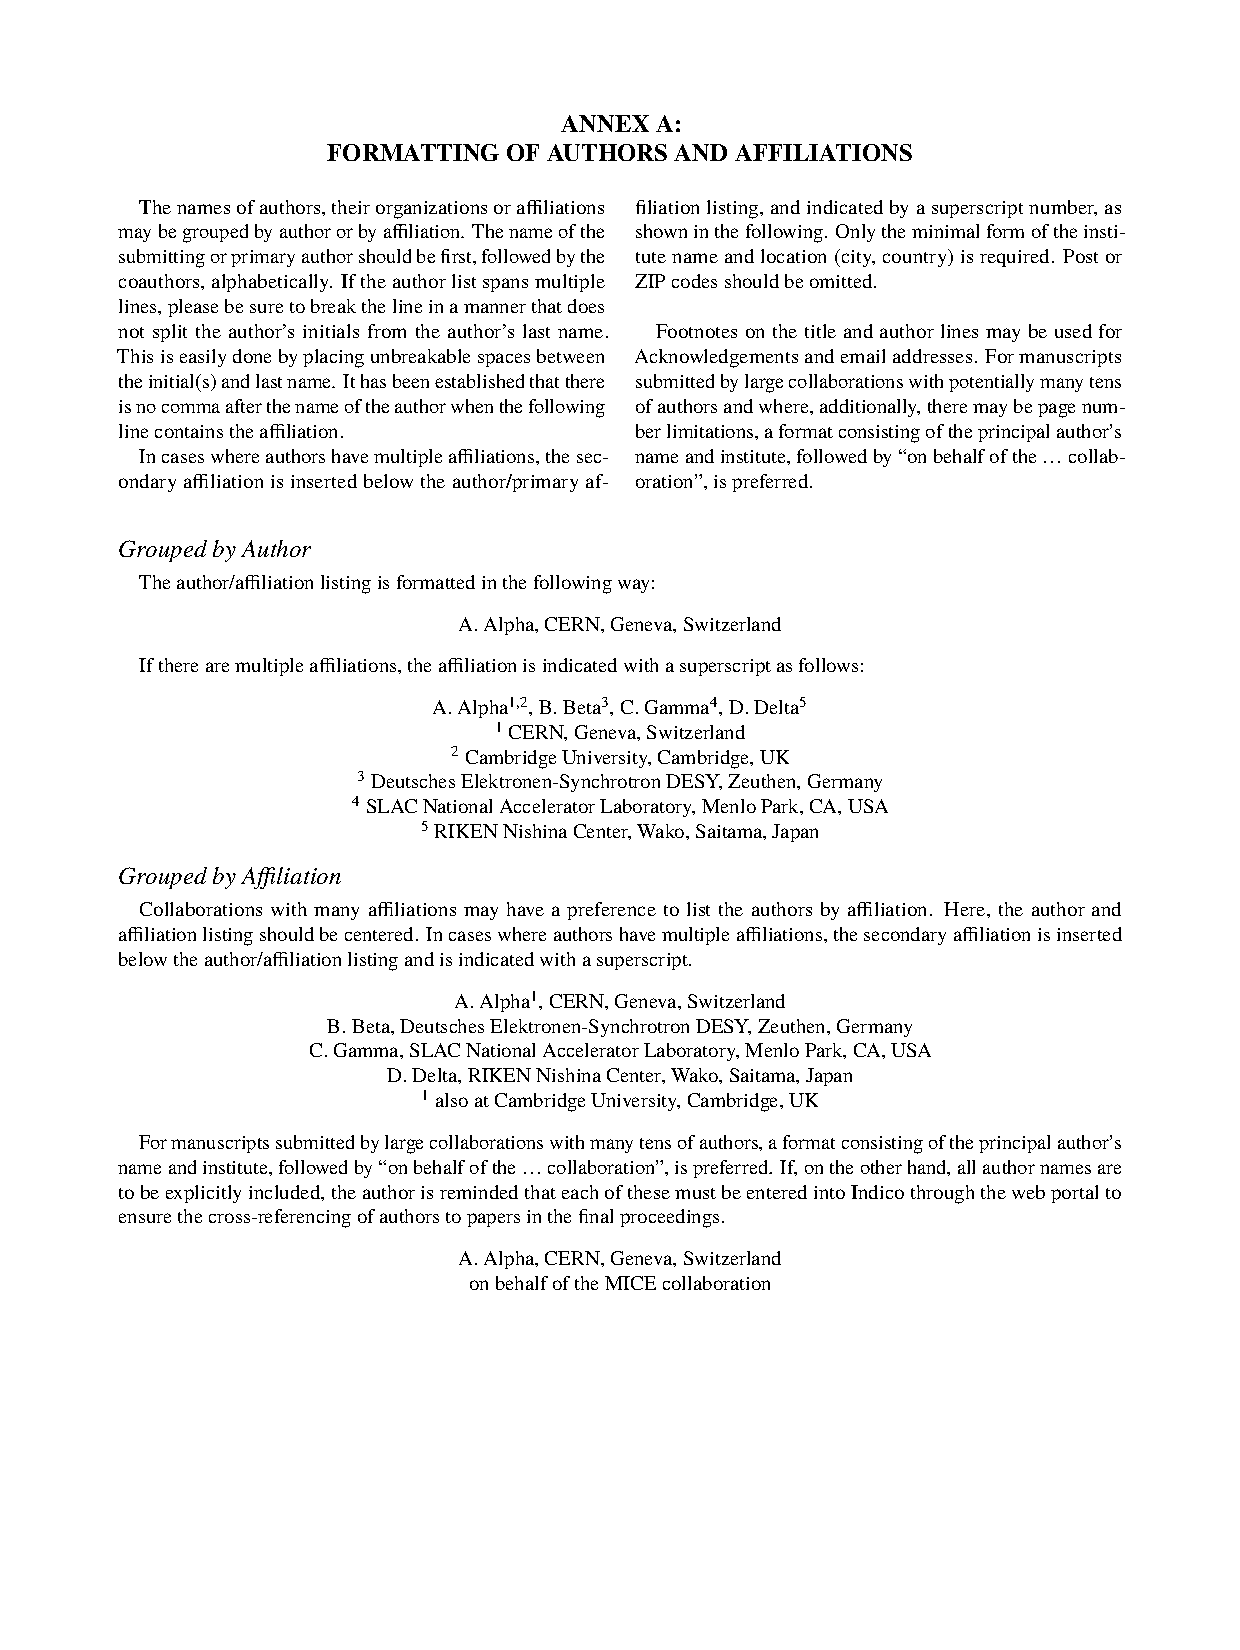
\includepdf[pages=-, noautoscale, offset=0pt 0pt]{jacow_latex_appendix_a.pdf}
%
% APPENDIX B: has been included in the source as »pdfpages« cannot 
%             import active links from included PDFs
%
\twocolumn[\vspace*{-1.8ex}%
		   \section{APPENDIX B: \\
		   			REFERENCE STYLE GUIDE AS APPLIED TO \NoCaseChange{JACoW} PAPERS, \\
		   			PERIODICALS AND OTHER WORKS}%
		   \vspace*{\baselineskip}]

\flushcolsend

\subsection{Formatting of Authors and Paper Titles}

The formatting of authors and paper titles is common to both proceedings’ volumes and journals and are outlined in the following.

\subsubsection{Author Listing}

Careful attention should be given to the placing of commas and the use of ‘and’ in the author list. For the case of three or more authors (as in Ref. [3]), a comma also follows the penultimate author. The preference for \textit{et al.} takes precedence when the number of authors is greater than six. See Table~\ref{tab:author-formatting} for a synopsis.
\begin{table}[!hbt]
   \centering
   \caption{Formatting Authors}
   \setlength\tabcolsep{2.5pt}
   \setlength\fboxsep{0pt}
   \begin{tabular}{p{25mm}l}
       \toprule
       \textbf{No. of Authors} & \textbf{Format} \\ 
       \midrule
           1		& A.\,T.\,Alpha,                  			\\
           2		& A.\,T.\,Alpha\fcolorbox{yellow}{yellow}{ and }B.\,Beta,					\\
           3 to 6	& A.\,T.\,Alpha, B.\,Beta\fcolorbox{yellow}{yellow}{, and }J.-P.\,Gamma,	\\ 
           >6		& A.\,T.\,Alpha\fcolorbox{yellow}{yellow}{~\textit{et al.}},				\\ 
           >6\,\,but\,\,with\,\,two \hphantom{>6 }\mbox{primary authors} 
           			& A.\,T.\,Alpha, B.\,Beta\fcolorbox{yellow}{yellow}{, \textit{et al.}}, 	\\
       \bottomrule
   \end{tabular}
   \label{tab:author-formatting}
\end{table}

\subsubsection{Paper Title}

As is modern practice in references, the title of the paper is written in sentence case, i.e., only the initial letter of the first word in the title is capitalized. Proper nouns, however, also have a capital. Capital letters appearing in acronyms likewise remain unaltered.

\subsection{Conference Proceedings}

The format for published JACoW proceedings papers is detailed in the following and can also be readily deduced from Refs. [1-5]. Use of the said style for references ensures a proper import into digital libraries and information sources such as INSPIRE, Scopus, and Google Scholar. Authors are also reminded to make a distinction between papers published in JACoW proceedings, which have page numbers and, in the case of recent publications, digital object identifiers (DOIs), and those papers that may have been presented at past JACoW conferences but were not published [6]. References to contributions presented at the same conference should be written as shown in Ref. [7].

\subsubsection{Conference Title}

The title of the proceedings is written in title case in italics using standard abbreviations, 
such as \textit{Int.} and \textit{Conf}. The preposition, “in”, in normal font, precedes the proceedings title. The abbreviated form of the conference is sufficient, e.g., in \textit{Proc. IPAC’24}. If the complete name of the conference is preferred to avoid possible ambiguities, then ISO~4 abbreviations may be applied, e.g., in \textit{Proc.13th Int. Comput. Accel. Phys. Conf. (ICAP’18)}.

\subsubsection{Conference Location and Month, Year}

The location, i.e., city, state (if applicable), and country of the conference venue, the month (three-letter abbreviation) and the year the conference took place, is then listed.

\subsubsection{Page Numbers and DOI}

Finally, details pertaining to the paper itself, such as mandatory page numbers, and the DOI, if existing, are listed in the given order. A mono-spaced font for the DOI is used to help distinguish it from normal text. The font for typesetting links in \LaTeX{} using the ‘\texttt{url}’ package 
is a monospaced (typewriter) font. To get a better distinction between »\texttt{O}« and~»\url{0}« the default font has been switched to »\texttt{newtxtt}«. The conference paper ID may be included in the absence of a DOI to facilitate a search through internet search engines. DOIs have been assigned to all JACoW publications since 2015, and IPAC2014. This list will be updated when older conferences are reprocessed with registered DOIs. The use of DOIs is strongly mandated, and an active hyperlink in the final PDF because in contrast to the standard »★https://★« links which might obsolete anytime, DOIs are designed to be permanent, they are a type of persistent identifier.

Use of the said style for references ensures a proper import into digital libraries and information sources such as INSPIRE, Scopus, and Google Scholar. Authors are also reminded to make a distinction between papers published in JACoW proceedings (which have page numbers and, in recent publications, DOIs) and those papers that may have been presented at past JACoW conferences but were not published~[6]. References to contributions presented at the same conference should be written as shown in Ref.~[7]; the wording “this conference” may be appended.

\subsection{Referencing Periodicals}

When referencing periodicals, special attention should be given to including all the necessary details: author names, paper title, journal, volume, page/article number, and year. The DOI should be included if available. These details should be formatted according to the style shown in Refs.~[8-12]. Journal abbreviations follow the ISO\,4 standard. References~[13, 14] are good sources for journal abbreviations. A set of selected journal abbreviations is listed in \textbf{APPENDIX~C}.

\subsection{Referencing Other Sources}

The IEEE style is also shown for papers that have been accepted or submitted for publication in periodicals~[15, 16], arXiv preprints~[17], online sources~[18-20], books~[21, 22], internal and technical reports~[23-27], theses~[28], handbooks and (reference) manuals~[29-31], patents~[32] and unpublished material~[33, 34].

\subsection{Alignment of References}

Entries to the \textbf{REFERENCES} section follow a hanging indent structure. In case of manual formatting of references, the value of `\texttt{x}' in the corresponding ★thebibliography★ command must be large enough to reserve sufficient space for the digits.
\begin{Tverb}
% Use for 10-99 references
   \begin{thebibliography}{99} 
% Use for  1-9 references
   \begin{thebibliography}{9}  
\end{Tverb}

\noindent%
This is automatically taken care of when using {Bib\LaTeX}.

\subsection{Paper Published in a Conference Proceedings}

The title of the paper is written in sentence case. References are typeset in \qty{9}{pt} size. The font for typesetting links in \LaTeX{} using the ‘\texttt{url}’ package is a mono-spaced (typewriter) font for DOIs (★\doi{}★) and URLs (★\url{}★). 
To get a better distinction between »\texttt{O}« and~»\url{0}« the default font has been switched to »\texttt{newtxtt}«. 

The DOI should be confined to within a single line rather than being split in arbitrary positions across multiple lines. This is achieved using the command ★\doi{}★, which measures the remaining space on the current line and inserts a line break if the DOI does not fit. In contrast to the functionality of the »★\url★« command, the »★\doi{10.xxx/yyyy}★« command places an active link to »★https://doi.org/10.xxx/yyyy★« in the PDF. This link redirects to the landing page of the publisher.

\setenumerate[1]{label=[\arabic*], topsep=0pt, leftmargin=16pt, itemsep=-1pt}
\begin{enumerate}\small
	\item A. Alpha, “Novel techniques for a future TeV electron accelerator”, 
		in \textit{Proc. IPAC’23}, Venice, Italy, May 2023, pp. 57-59. \\ \href{https://doi.org/10.18429/JACoW-IPAC2023}%
		     {\texttt{{doi:10.18429/JACoW-IPAC2023-PAPERID}}}

	\item A. Alpha and B. T. Beta, “An overview of modern control systems”, 
		in \textit{Proc. ICALEPCS’23}, Cape Town, South Africa, Oct. 2023, pp. 57-59. \\ \href{https://doi.org/10.18429/JACoW-ICALEPCS2023}%
		     {\texttt{doi:10.18429/JACoW-ICALEPCS2023-PAPERID}}

	\item A. Alpha, B. T. Beta, and J.-P. Gamma, “Compact light sources”, 
		in \textit{ Proc. FLS’23}, Lucerne, Switzerland, Aug.-Sep 2023, pp. 57-59. \\ \href{https://doi.org/10.18429/JACoW-FLS2023}%
		     {\texttt{doi:10.18429/JACoW-FLS2023-PAPERID}}

	\item A. Alpha \textit{et al.}, “Novel techniques for future TeV electron accelerators”, 
		in \textit{Proc. LINAC’24}, Chicago, IL, USA, Aug 2024, pp. 57-59. \\
		\href{https://doi.org/10.18429/JACoW-LINAC2024}%
		    {\texttt{doi:10.18429/JACoW-LINAC2024-PAPERID}}

	\item A. Alpha, B. T. Beta, \textit{et al.}, “Status of Cyclotrons around the world”, 
		in \textit{Proc. Cyclotrons’22}, Beijing, China Dec. 2022, pp. 57-59. \\
		\href{https://doi.org/10.18429/JACoW-CYCLOTRONS2022}%
		     {\texttt{doi:10.18429/JACoW-CYCLOTRONS2022-PAPERID}}
\end{enumerate}

\subsection{Unpublished Paper from a Previous Conference}

The conference name is given in normal font. The paper ID may be given if material supplementing the proceedings exists on the JACoW website, e.g., PDF of talk.
\begin{enumerate}[resume*]\small
	\item A. Alpha, “An interesting talk but paper not submitted”, presented at IPAC’14, Dresden, Germany, Jun. 2014, paper MOP057, unpublished. 
\end{enumerate}

\subsection{Paper Presented at the Current Conference}

For papers at the current conference the conference name is given in normal upright font preceded by ‘presented at’:
\begin{enumerate}[resume*]\small
	\item  A. Alpha and B. T. Beta, “Title of talk or poster presented at this conference”, 
		presented at IPAC’25, Taipei, Taiwan, Jun. 2025, paper MOAB01, this conference.
\end{enumerate}

\subsection{Published in a Periodical}

If journals are paginated by volume, the issue number is optional. 
The month of publication is optional.

\begin{enumerate}[leftmargin=22pt, resume*]\small
	\item A. Alpha \textit{et al.}, “Title of paper published in journal”, 
		\textit{Phys. Rev. Lett.}, vol. 114, no. 5, p. 050511, Feb. 2014. 
		\href{https://doi.org/10.1103/PhysRevLett.114.050511}%
		     {\texttt{doi:10.1103/PhysRevLett.114.050511}}

	\item A. Alpha, “New techniques in laser wakefield accelerators”, 
		\textit{Phys. Rev. Accel. Beams}, vol. 22, p. 014601, Jan. 2019. \\ \href{https://doi.org/10.1103/PhysRevAccelBeams.22.014601}%
		     {\texttt{doi:10.1103/PhysRevAccelBeams.22.014601}}

	\item A. Alpha, B. Beta, C. Gamma, D. Delta, E. Epsilon, and Z.~Zeta, 
		“Exotic beams”, \textit{Phys. Rev. Spec. Top. Accel. Beams}, vol. 1, p. 013501, May. 1998.	\\ \href{https://doi.org/10.1103/PhysRevSTAB.1.013501}%
		     {\texttt{doi:10.1103/PhysRevSTAB.1.013501}}

	\item A. Alpha \textit{et al.}, 
		“Low dose irradiation impact on modern silicon detectors”, 
		\textit{Nucl. Instrum. Methods Phys. Res. A}, vol. 773, pp. 1-7, 2015. \\ \href{https://doi.org/10.1016/j.nima.2014.11.022}%
		     {\texttt{doi:10.1016/j.nima.2014.11.022}}

	\item A. Alpha, B. Beta, and C. Gamma, 
		“Temporal correlations of x-ray free electron lasers”, 
		\textit{Optics Express}, vol. 33, no. 8, pp. 17884-17885, 2012. \\
		\href{https://doi.org/10.1364/OE.564805}%
			 {\texttt{doi:10.1364/OE.564805}}
\end{enumerate}

\subsection{Journal Abbreviations}

The following are good sources of journal abbreviations:
\begin{enumerate}[leftmargin=22pt, resume*]\small
	\item M. Wrochna, “List of Title Word Abbreviations”,
		\nolinkurl{https://marcinwrochna.github.io/abbrevIso/}

	\item  Kevin Lindstrom, Science and Engineering Journal Abbreviations, Woodward Library, 
		The University of British Columbia, BC, Canada, 
		\nolinkurl{https://woodward.library.ubc.ca/research-help/journal-abbreviations/}
\end{enumerate}

\subsection{Accepted for Publication}

\begin{enumerate}[leftmargin=22pt, resume*]
	\item J. B. Good, “Title of paper accepted for publication”, 
		\textit{Phys. Rev. Lett.}, to be published.
\end{enumerate}

\subsection{Submitted for Publication}

The name of the periodical is not listed.

\begin{enumerate}[leftmargin=22pt, resume*]
	\item G. D. Read, “Title of paper”, submitted for publication.
		arXiv Preprint

	\item  A. Alpha, “Title of arXiv preprint”, Jan. 2025. 
		\href{https://doi.org/10.48550/arXiv.2501.10602}%
			 {\texttt{doi:10.48550/arXiv.2501.10602}}
\end{enumerate}

\subsection{Online Source}

Note that hyperlinks to non-DOI URLs are prohibited.

\begin{enumerate}[leftmargin=22pt, resume*]
	\item JACoW, \url{https://www.jacow.org}

	\item EPICS, \url{https://www.epics-controls.org}

	\item Principal Component Analysis, \\ 
		\url{https://en.wikipedia.org/wiki/Principal_component_analysis}
\end{enumerate}

\subsection{Citations to Books}
A reference to a chapter in a book:
\begin{enumerate}[leftmargin=22pt, resume*]
	\item A. Alpha and B. Beta, 
		“Title of chapter in the book”, in \textit{Title of Book}, 
		R Mars, Ed. New York, NY, USA: Wiley, 1994, pp. 42-48.
\end{enumerate}

A reference to a book:
\begin{enumerate}[leftmargin=22pt, resume*]
	\item A. Alpha, \textit{Title of Book}. 
		Cambridge, MA, USA: MIT Press, 1986.
\end{enumerate}

\subsection{Internal Report}

\begin{enumerate}[leftmargin=22pt, resume*]
	\item A. Alpha \textit{et al.}, “Title of report”, CERN, Geneva, Switzerland, 
		Rep. CERN-2012-333, Oct. 2012.

	\item A. Alpha, B. Beta, C. Gamma, D. Delta, E. Epsilon, and Z.~Zeta, 
		“Title of report”, SLAC National Accelerator Laboratory, Menlo Park, CA, USA, Rep. SLAC-REP-474, May 1996.
\end{enumerate}

\flushcolsend
\subsection{Technical Report}

\begin{enumerate}[leftmargin=22pt, resume*]
	\item SLS-2 Conceptional Design Report, 
		A. Streun, Ed., Paul Scherrer Institute, Villigen, Switzerland, Rep. 17-03, Dec.~2017. \url{https://www.dora.lib4ri.ch/psi/item/psi:34977}

	\item \textit{Advanced Photon Source Upgrade Project Final Design Report}, 
		Argonne National Laboratory, Lemont, IL, USA, Rep.~APSU-2.01-RPT-003, May 2019. \url{https://publications.anl.gov/anlpubs/2019/07/153666.pdf} 

	\item SwissFEL Conceptual Design Report, 2\textsuperscript{nd} ed., 
		R. Ganter, Ed., Paul Scherrer Institute, Villigen, Switzerland, Rep. 10-04, Apr. 2012. \url{https://www.dora.lib4ri.ch/psi/item/psi:41664} 
		
\end{enumerate}

\subsection{Thesis}

\begin{enumerate}[leftmargin=22pt, resume*]
	\item A. Student, “Title of thesis”, Ph.D. thesis, Phys. Dept., 
		Karlsruher Institut für Technologie, Karlsruhe, Germany, 2014.
\end{enumerate}

\subsection{Handbook}

\begin{enumerate}[leftmargin=22pt, resume*]
	\item Name of Handbook, 2nd ed., Name of Company, Country, 
		Apr. 2024, pp. 34-52, \url{http://www.xyz.com/etc}

	\item Motorola Semiconductor Handbook, Motorola Semiconductor Products Inc., 
		Phoenix, AZ, USA, Nov. 2021, \url{https://www.motorola.com/etc}
\end{enumerate}

\subsection{Reference, Manual}

\begin{enumerate}[leftmargin=22pt, resume*]
	\item \textit{IEEE Editorial Style Manual for Authors},
		IEEE Periodicals, Piscataway,
		NJ, USA, Mar. 2025. \\
		\url{https://docs.google.com/document/d/1OalFYqVfxKKMelF79U3B93SjmIEiTnJC12wPJrKeSDM/}
\end{enumerate}

\subsection{Patents}

\begin{enumerate}[leftmargin=22pt, resume*]
	\item  A. N. Inventor, “Title of patent”, 
		<Patent Authority and No.>, Jan. 20, 2016. \\[3pt]
		A. N. Inventor, “Title of patent”, 
		<Patent Authority>, patent pending.

\end{enumerate}

\subsection{Unpublished Work and Private Communication}

\begin{enumerate}[leftmargin=22pt, resume*]
	\item P. Neptune, “Title of paper”, unpublished.
	
	\item P. Uranus, private communication, Jun. 2015.
\end{enumerate}

\newpage
%
% Appendix C: Jan's original will be included
%
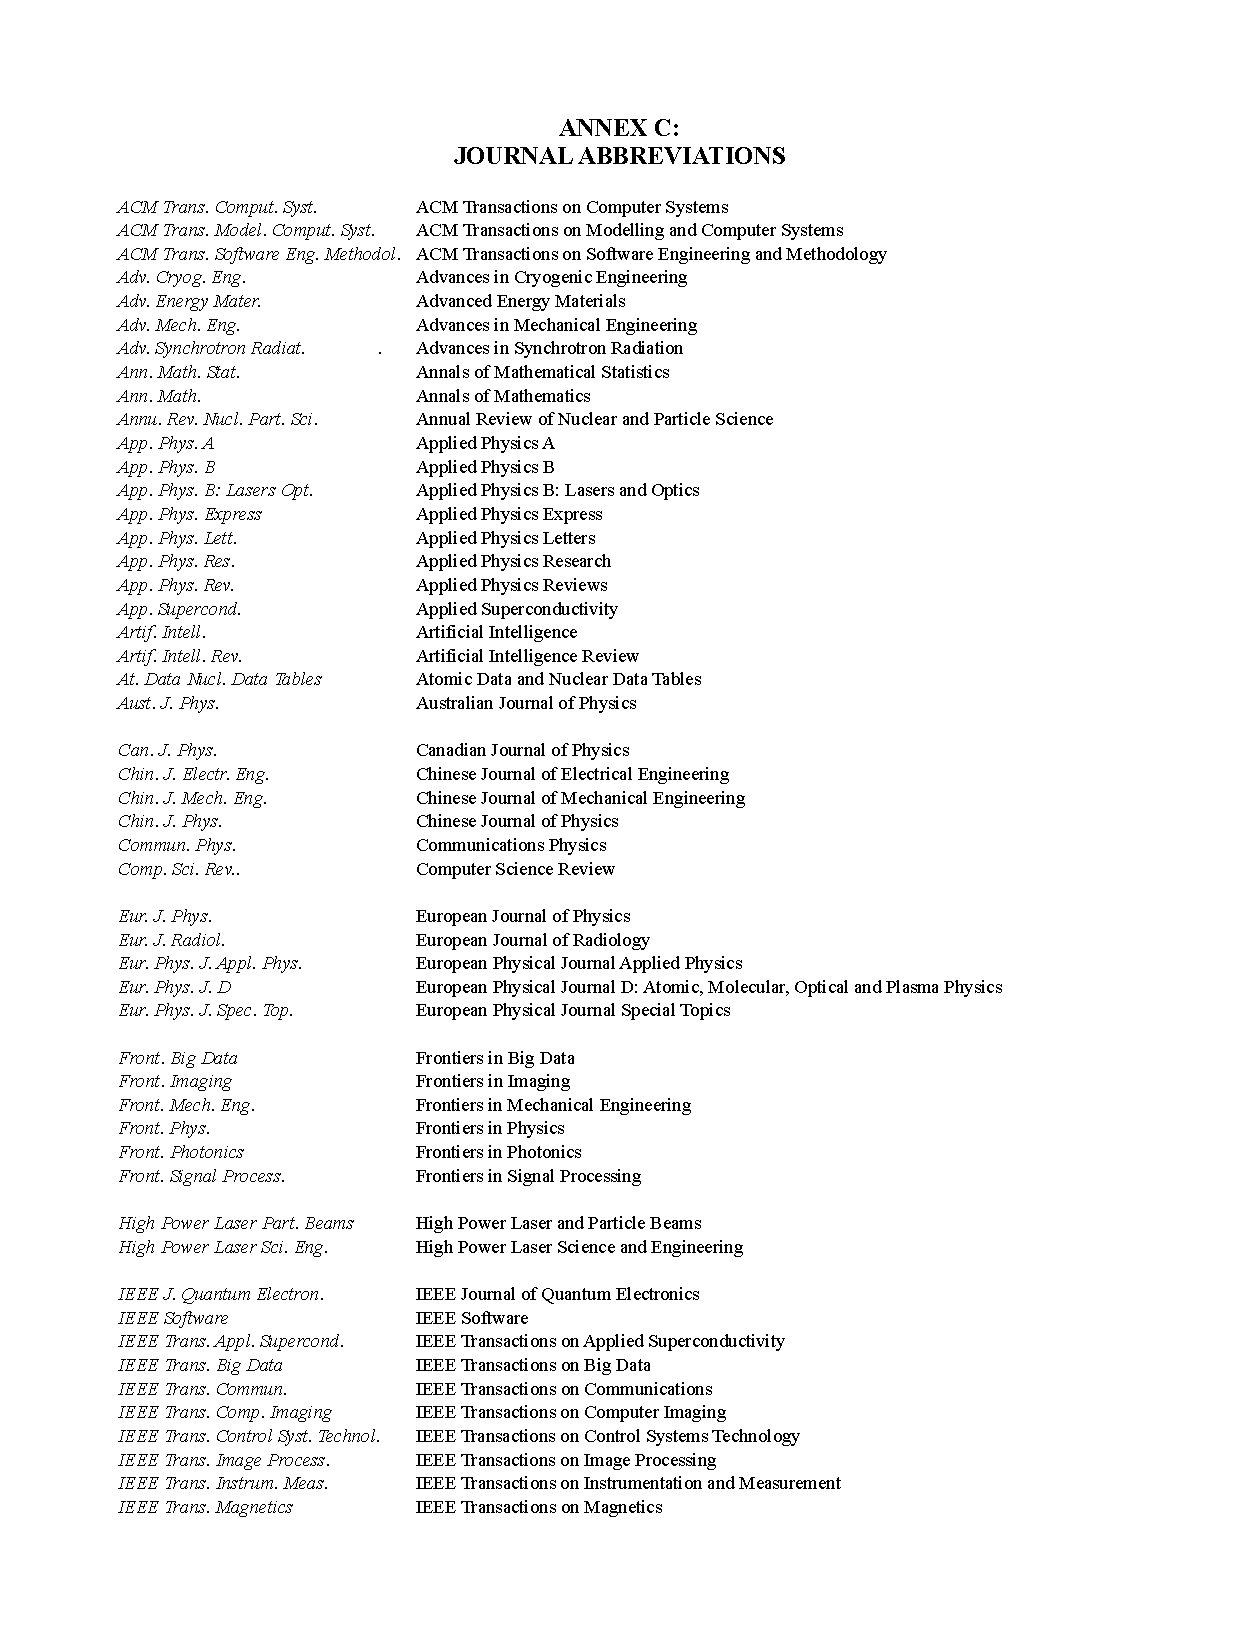
\includepdf[pages=-, noautoscale, offset=0pt 0pt]{jacow_latex_appendix_c.pdf}

\end{document}
